% Options for packages loaded elsewhere
\PassOptionsToPackage{unicode}{hyperref}
\PassOptionsToPackage{hyphens}{url}
%
\documentclass[
  12pt,
]{book}
\usepackage{lmodern}
\usepackage{amsmath}
\usepackage{ifxetex,ifluatex}
\ifnum 0\ifxetex 1\fi\ifluatex 1\fi=0 % if pdftex
  \usepackage[T1]{fontenc}
  \usepackage[utf8]{inputenc}
  \usepackage{textcomp} % provide euro and other symbols
  \usepackage{amssymb}
\else % if luatex or xetex
  \usepackage{unicode-math}
  \defaultfontfeatures{Scale=MatchLowercase}
  \defaultfontfeatures[\rmfamily]{Ligatures=TeX,Scale=1}
\fi
% Use upquote if available, for straight quotes in verbatim environments
\IfFileExists{upquote.sty}{\usepackage{upquote}}{}
\IfFileExists{microtype.sty}{% use microtype if available
  \usepackage[]{microtype}
  \UseMicrotypeSet[protrusion]{basicmath} % disable protrusion for tt fonts
}{}
\makeatletter
\@ifundefined{KOMAClassName}{% if non-KOMA class
  \IfFileExists{parskip.sty}{%
    \usepackage{parskip}
  }{% else
    \setlength{\parindent}{0pt}
    \setlength{\parskip}{6pt plus 2pt minus 1pt}}
}{% if KOMA class
  \KOMAoptions{parskip=half}}
\makeatother
\usepackage{xcolor}
\IfFileExists{xurl.sty}{\usepackage{xurl}}{} % add URL line breaks if available
\IfFileExists{bookmark.sty}{\usepackage{bookmark}}{\usepackage{hyperref}}
\hypersetup{
  pdftitle={Dr.~Duncan Hull, University of Manchester},
  hidelinks,
  pdfcreator={LaTeX via pandoc}}
\urlstyle{same} % disable monospaced font for URLs
\usepackage{longtable,booktabs}
\usepackage{calc} % for calculating minipage widths
% Correct order of tables after \paragraph or \subparagraph
\usepackage{etoolbox}
\makeatletter
\patchcmd\longtable{\par}{\if@noskipsec\mbox{}\fi\par}{}{}
\makeatother
% Allow footnotes in longtable head/foot
\IfFileExists{footnotehyper.sty}{\usepackage{footnotehyper}}{\usepackage{footnote}}
\makesavenoteenv{longtable}
\usepackage{graphicx}
\makeatletter
\def\maxwidth{\ifdim\Gin@nat@width>\linewidth\linewidth\else\Gin@nat@width\fi}
\def\maxheight{\ifdim\Gin@nat@height>\textheight\textheight\else\Gin@nat@height\fi}
\makeatother
% Scale images if necessary, so that they will not overflow the page
% margins by default, and it is still possible to overwrite the defaults
% using explicit options in \includegraphics[width, height, ...]{}
\setkeys{Gin}{width=\maxwidth,height=\maxheight,keepaspectratio}
% Set default figure placement to htbp
\makeatletter
\def\fps@figure{htbp}
\makeatother
\setlength{\emergencystretch}{3em} % prevent overfull lines
\providecommand{\tightlist}{%
  \setlength{\itemsep}{0pt}\setlength{\parskip}{0pt}}
\setcounter{secnumdepth}{5}
\usepackage{booktabs}
\ifluatex
  \usepackage{selnolig}  % disable illegal ligatures
\fi
\usepackage[]{natbib}
\bibliographystyle{apalike}

\title{Dr.~Duncan Hull, University of Manchester}
\author{}
\date{\vspace{-2.5em}}

\begin{document}
\maketitle

{
\setcounter{tocdepth}{1}
\tableofcontents
}
\hypertarget{hello}{%
\chapter*{Hello!}\label{hello}}
\addcontentsline{toc}{chapter}{Hello!}

\begin{figure}

{\centering \includegraphics[width=0.9\linewidth]{images/duncan hull unplashed} 

}

\caption{This is me. Background photo by \href{https://unsplash.com/@slidebean}{slidebean} on \href{https://unsplash.com}{unsplash.com}, a source of \href{https://unsplash.com/license}{freely-usable images}.}\label{fig:unsplashed-fig}
\end{figure}



Hello and welcome to the \href{https://www.cs.manchester.ac.uk/}{Department of Computer Science} at the \href{https://www.manchester.ac.uk}{University of Manchester}. My name is Duncan and I'm a lecturer (≈ \href{https://en.wikipedia.org/wiki/Assistant_professor}{Assistant Professor}) here with responsibility for managing our \href{https://www.cs.manchester.ac.uk/study/undergraduate/industrial-experience/}{Industrial Experience} (IE) program. This elective course has \protect\hyperlink{employability}{around 100} students every year working in paid employment for the penultimate (``sandwich'') year-in-industry of their undergraduate degrees. 🥪🎓

I \href{http://www.cs.man.ac.uk/~hulld/teaching.html}{teach} undergraduate \& postgraduate students, supervise tutorials \& projects while serving as \href{http://studentnet.cs.manchester.ac.uk/employment/placement/}{employability tutor}. I'm interested in methods that can \href{http://www.cs.man.ac.uk/~hulld/research.html}{improve teaching, learning and the student experience} using techniques like \href{https://www.cdyf.me}{coding your future}, \href{https://www.cs.manchester.ac.uk/connect/business-engagement/industrial-mentoring/}{industrial mentoring}, \href{https://sigcse.cs.manchester.ac.uk/}{journal clubbing}, \href{http://www.cs.man.ac.uk/~hulld/coding-their-future.html}{working with local schools}, \protect\hyperlink{wikipedia}{Wikipedia editing}, and \protect\hyperlink{tuningcomplete}{live music}. 🎸

If you are an \href{http://www.cs.man.ac.uk/~hulld/employers.html}{employer} who would like to recruit a summer intern, placement student or graduate please \href{http://www.cs.man.ac.uk/~hulld/contact.html}{get in touch}. During term time, we edit and highlight some of the best opportunities for students in a weekly newsletter known as the \href{https://waggle.cs.manchester.ac.uk/waggle/about}{Wednesday Waggle} which goes out to over 1000 undergraduate and postgraduates in Computer Science. 🐝

\hypertarget{full-stack-teaching}{%
\section*{Full stack teaching}\label{full-stack-teaching}}
\addcontentsline{toc}{section}{Full stack teaching}

Regardless of the age or the stage, I enjoy the challenges of teaching and have taught english, maths, science and engineering to primary \& secondary school children (\href{https://en.wikipedia.org/wiki/K\%E2\%80\%9312}{K--12}), undergraduates \& postgraduates. In 2011, I completed a \href{https://en.wikipedia.org/wiki/Postgraduate_Certificate_in_Education}{Postgraduate Certificate in Education} (PGCE) at the \href{https://www.bath.ac.uk/}{University of Bath} and worked as a high school science teacher in co-educational \href{https://en.wikipedia.org/wiki/State-funded_schools_(England)}{non-selective state-funded schools} in Swindon, Shaftesbury and Stockport before returning to higher education. As well as teaching in the UK I have been fortunate enough to teach in India, Japan and America too. 🇬🇧🇮🇳🇯🇵🇺🇸

\hypertarget{whats-the-story}{%
\section*{What's the story?}\label{whats-the-story}}
\addcontentsline{toc}{section}{What's the story?}

Born in \href{https://en.wikipedia.org/wiki/Bath,_Somerset}{Bath, Somerset} and raised using a \href{https://en.wikipedia.org/wiki/West_Country}{secret West Country recipe}, \href{https://uk.linkedin.com/in/duncanhull}{my story} is a mixture of Natural Sciences (\href{http://www.plantsciences.manchester.ac.uk/}{Plant Sciences, BSc}), Computer Science (\href{http://www.cs.man.ac.uk/~hulld/msc2003.html}{MSc} \& PhD) and software engineering. I've worked as a consultant and software developer for various organisations including \href{https://en.wikipedia.org/wiki/BBC_Monitoring}{BBC Monitoring}, the \href{https://en.wikipedia.org/wiki/Ford_Motor_Company}{Ford Motor Company} and the \href{https://en.wikipedia.org/wiki/National_Health_Service}{National Health Service} (NHS). While working on \href{https://en.wikipedia.org/wiki/Apache_Taverna}{Apache Taverna} and \href{https://en.wikipedia.org/wiki/MyGrid}{myGrid} I completed a \href{https://ethos.bl.uk/OrderDetails.do?uin=uk.bl.ethos.497578}{PhD} at the University of Manchester. This was followed by a \href{https://en.wikipedia.org/wiki/Postdoctoral_researcher}{postdoc} at the \href{https://www.mib.manchester.ac.uk/}{Manchester Institute of Biotechnology} (MIB) working on the \href{http://www.nactem.ac.uk/pathtext/}{Refine project} and a stint as a software engineer of \href{https://en.wikipedia.org/wiki/ChEBI}{Chemical Entities of Biological Interest} (ChEBI) at the \href{https://en.wikipedia.org/wiki/European_Bioinformatics_Institute}{European Bioinformatics Institute} in Cambridge, UK. 🧬🇪🇺

\hypertarget{toolbox}{%
\section*{Toolbox}\label{toolbox}}
\addcontentsline{toc}{section}{Toolbox}

This website\footnote{last updated 09 April, 2021} is built using \href{https://bookdown.org}{bookdown} with \href{https://rmarkdown.rstudio.com/}{R markdown}, the \href{https://en.wikipedia.org/wiki/R_(programming_language)}{R language}, \href{https://www.gitbook.com}{gitbook}, \href{https://en.wikipedia.org/wiki/JavaScript}{JavaScript}, \href{https://en.wikipedia.org/wiki/Knitr}{knitr}, \href{https://en.wikipedia.org/wiki/LaTeX}{LaTeX}, \href{https://pandoc.org/}{Pandoc}, \href{https://rstudio.com/}{RStudio} and TLC. Thanks to \href{https://yihui.org}{Yihui Xie} and his collaborators for the handy tools and excellent documentation. The \href{https://github.com/dullhunk/hulled}{source is available on github} and the documentation in \emph{\href{https://bookdown.org/yihui/bookdown/}{Authoring Books and Technical Documents with R Markdown}}. If you're viewing this page on an iPhone or iPad, there is \href{https://github.com/rstudio/bookdown/issues/60}{known bug with the menu bar at the top of this page} which means the menu might not display properly. These pages are also available \href{http://www.cs.man.ac.uk/~hulld/duncan-hull.pdf}{in one single pdf file} and \href{http://www.cs.man.ac.uk/~hulld/duncan-hull.epub}{and an ebook}.

\hypertarget{get-a-life}{%
\section*{Get a life!}\label{get-a-life}}
\addcontentsline{toc}{section}{Get a life!}

When I get the time I like to \href{https://en.wikipedia.org/wiki/Baritone}{sing baritone}, practice my \protect\hyperlink{tuningcomplete}{embarrassing dad dance} moves, \href{http://beelife.cs.manchester.ac.uk/}{look after bees} and butcher the greek language, preferably on a beach in Greece. Άντε γειά! 🏖️🇬🇷

\hypertarget{teaching}{%
\chapter{Students}\label{teaching}}

I teach, mentor, tutor, lecture on and supervise a variety of undergraduate and postgraduate courses. You can find me online during office hours, in the labs, my office and the lecture theatre. 🎭

\begin{figure}

{\centering 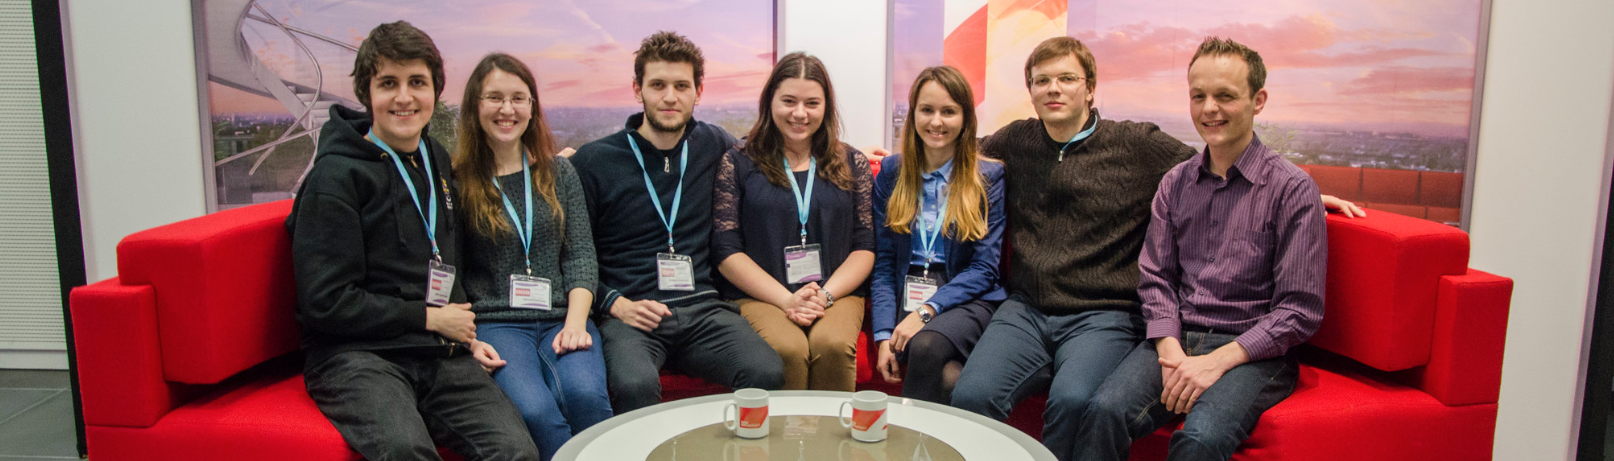
\includegraphics[width=1\linewidth]{images/bbcbreakfastsofa} 

}

\caption{Posing on the \href{https://en.wikipedia.org/wiki/BBC_Breakfast}{BBC Breakfast} red sofa with the winning team of the BBC / Barclays University Technology Challenge (UTC) in \href{https://en.wikipedia.org/wiki/MediaCityUK}{MediaCityUK}, Salford}\label{fig:unnamed-chunk-1}
\end{figure}



\hypertarget{allyears}{%
\section{All years: Debug your CV}\label{allyears}}

If you'd like to debug your CV, application form, covering letter and job search etc, read \href{https://www.cdyf.me/debugging.html}{debugging your future} \citep{debugyourfuture} and \href{https://www.cdyf.me/sampling.html}{reading their future} \citep{readingtheirfuture}, especially if you haven't written a CV (two pages), résumé (one page) or LinkedIn profile before. Once you've done this you can send me any relevant documentation and then:

\begin{itemize}
\tightlist
\item
  Drop-in to my weekly one-to-one CV clinics for Computer Science students in LF25 during term-time during my open office hours: Tuesday from 10am to midday
\item
  Get feedback on your CV from as many other people as possible, because ``\href{https://en.wikipedia.org/wiki/Linus\%27s_law}{given enough eyeballs, all bugs are shallow}'' \citep{Raymond1999}
\end{itemize}

Outside of term time, it's best to book a debugging appointment. 🐛

\hypertarget{year1}{%
\section{First year students}\label{year1}}

If you're in your first year of study, I serve as:

\begin{itemize}
\tightlist
\item
  Academic staff member for \href{https://studentnet.cs.manchester.ac.uk/ugt/COMP10120/syllabus/}{First year team projects: COMP101} led by \href{http://www.cs.man.ac.uk/~sattler/}{Ulrike Sattler} \citep{COMP10120}, see the \href{http://latex4year1.netlify.app}{getting started with LaTeX lab manual}
\item
  Mentor and tutor to one group of six first year students
\item
  Organiser of first year guest lectures, which mostly run in the second semester, February to May
\end{itemize}

\hypertarget{year2}{%
\section{Second year students}\label{year2}}

If you're in your second year, I serve as:

\begin{itemize}
\tightlist
\item
  Course leader for \href{https://studentnet.cs.manchester.ac.uk/ugt/COMP23311/syllabus/}{second year software engineering: COMP23311}, a course designed by \href{http://www.cs.man.ac.uk/~embury/}{Suzanne Embury} \citep{COMP23311, git}
\item
  Organiser of the labs for the \href{https://www.cs.manchester.ac.uk/connect/business-engagement/industrial-mentoring/}{software engineering mentoring program}
\item
  Course leader for \href{https://www.cdyf.me/}{Coding your Future: COMP2CARS} a course designed by me for (primarily) second year students to design, build, test and debug their futures in computing.
\end{itemize}

Previously I served as \href{https://studentnet.cs.manchester.ac.uk/ugt/year2/}{second year tutor} from 2016 through to 2020.

\hypertarget{penultimate}{%
\section{Penultimate year students}\label{penultimate}}

If you're on placement during your penultimate year (your last-but-one), I serve as:

\begin{itemize}
\tightlist
\item
  Course leader for ``with industrial experience'' (IE), an elective and intercalated year in industry.
\item
  Year tutor for students on placement, either face to face or via telecon
\end{itemize}

\hypertarget{finalyear}{%
\section{Final year students}\label{finalyear}}

If you're in your final year of study, you'll find me:

\begin{itemize}
\tightlist
\item
  Supervising final year educational projects based in secondary schools in Greater Manchester, see \href{http://www.cs.man.ac.uk/~hulld/coding-their-future.html}{coding their future}. \citep{computinged} 👩‍💻👨‍💻
\end{itemize}

\hypertarget{masters}{%
\section{Masters students}\label{masters}}

If you're doing a Masters degree, you'll find me:

\begin{itemize}
\tightlist
\item
  Leading the course on \href{http://studentnet.cs.manchester.ac.uk/pgt/COMP60532/syllabus/}{Principles of Digital Biology} which covers \href{https://en.wikipedia.org/wiki/Bioinformatics}{Bioinformatics}, \href{https://en.wikipedia.org/wiki/Computational_biology}{Computational Biolgy} and a bit of \href{https://en.wikipedia.org/wiki/Health_informatics}{medical informatics} 🧬
\item
  Supervising \href{https://www.cs.manchester.ac.uk/study/masters/}{Master of Science} projects in Computer Science and Data Science. \citep{r4ds} This typically involves various combinations of Wikipedia, Wikdata, \href{https://en.wikipedia.org/wiki/SPARQL}{SPARQL} \citep{ducharme} and chatbots. 🤖 \citep{myca}
\end{itemize}

\hypertarget{phds}{%
\section{PhD students}\label{phds}}

If you've got any interesting PhD research ideas you like to pitch to me, particularly if they involve \href{https://sigcse.cs.manchester.ac.uk}{computer science education} or professional issues, I'm all ears! 👂

\hypertarget{extracurricular}{%
\section{Extracurricular}\label{extracurricular}}

Outside all of the above, I also get involved in:

\begin{itemize}
\tightlist
\item
  Organising, facilitating and promoting extra-curricular activities such as \href{https://en.wikipedia.org/wiki/Hackathon}{hackathons} \citep{Briscoe, Warner2017} and \href{https://en.wikipedia.org/wiki/Edit-a-thon}{edit-a-thons}. \citep{goodbadugly, troubled, findingada2019} These usually occur off-timetable, for example Wednesday afternoons, evenings and weekends.
\item
  Judging competitions such as \href{https://www.studenthack.com}{studenthack.com} and \href{https://greatunihack.com}{greatunihack.com} since 2014. These two hackathons are organised by \href{https://www.unicsmcr.com/}{UniCS}, a student-led tech society formed by the merger of HackSoc (computer geekery) and CSSoc (socialising). Many other hackathons exist, they are usually aimed at beginners looking to learn new skills, rather than experts looking to compete. \citep{Briscoe, hafb}
\end{itemize}

\hypertarget{employers}{%
\chapter{Employers}\label{employers}}

We work with a wide range of employers from the smallest bedroom startup to the worlds largest multi-national corporations, and are always looking for more organisations that can offer our students a stimulating working environment. According to \href{https://www.highfliers.co.uk}{highfliers.co.uk}, the University of Manchester is the most targeted University in the UK by the \href{https://www.top100graduateemployers.com}{Times Top 100 Graduate Employers}. \citep{times100, highfliers2020, Birchall2019} We can still do better, for example by engaging with a more diverse group of employers, especially those in Manchester and the \href{https://northernpowerhouse.gov.uk/}{Northern Powerhouse}, see \href{https://git.io/manc}{git.io/manc}. \citep{gitmanc, londonvstherest, hebdenbridge, manhattanchester, manchattan}

\begin{figure}

{\centering 
\includegraphics[width=1\linewidth]{images/industry-club-wide} 

}

\caption{Any employer recruiting our students is welcome to join our industry club, see details below}\label{fig:unnamed-chunk-2}
\end{figure}

\hypertarget{recruiting}{%
\section{Recruiting students}\label{recruiting}}

If you are recruiting computer scientists and software engineers as a summer interns, placement students or as graduates please get in touch with me or \href{https://uk.linkedin.com/in/mabel-yau}{Mabel Yau} (careers and placements officer). We typically have around 250 undergraduate students graduating annually, alongside a smaller number of Masters and PhD students. The \href{https://www.ucas.com/ucas/tariff-calculator}{entry tariff} of our students (A* AA including A* in mathematics) is comparable to other leading Computer Science (CS) departments in \href{https://en.wikipedia.org/wiki/Russell_Group}{Russell Group} universities as shown in the table below.

\begin{longtable}[]{@{}lll@{}}
\toprule
Institute & UCAS entry tariff & CS Students per year\tabularnewline
\midrule
\endhead
\href{https://www.undergraduate.study.cam.ac.uk/courses/computer-science}{University of Cambridge} & A* A* A & \textasciitilde100\tabularnewline
\href{https://www.ucl.ac.uk/prospective-students/undergraduate/degrees/computer-science-bsc/2020}{University College London} & A* A* A & \textasciitilde150\tabularnewline
\href{https://www.imperial.ac.uk/computing/prospective-students/courses/ug/beng-meng-computing/}{Imperial College London} & A* A* A & \textasciitilde200\tabularnewline
\href{https://www.manchester.ac.uk/study/undergraduate/courses/2019/00560/bsc-computer-science/}{University of Manchester} & A* A A & \textasciitilde250\tabularnewline
\href{http://www.ox.ac.uk/admissions/undergraduate/courses-listing/computer-science}{University of Oxford} & A* A A & \textasciitilde50\tabularnewline
\bottomrule
\end{longtable}

A demographic breakdown of our students in Computer Science is show in Figure \ref{fig:pie-fig}. If you are looking to recruit science and engineering students from other disciplines like \href{https://www.physics.manchester.ac.uk/}{Physics}, \href{https://www.maths.manchester.ac.uk/}{Maths}, \href{https://www.chemistry.manchester.ac.uk/}{Chemistry}, Mechnical, Aerospace \& Civil Engineering (\href{https://www.mace.manchester.ac.uk/}{MACE}), \href{https://www.materials.manchester.ac.uk/}{Materials Science} and Electrical \& Electronic Engineering (\href{https://www.eee.manchester.ac.uk/}{EEE}) you should talk to:

\begin{itemize}
\tightlist
\item
  staff in those departments and/or\\
\item
  the central careers service at \href{http://www.careers.manchester.ac.uk/}{careers.manchester.ac.uk}
\end{itemize}

\begin{figure}

{\centering 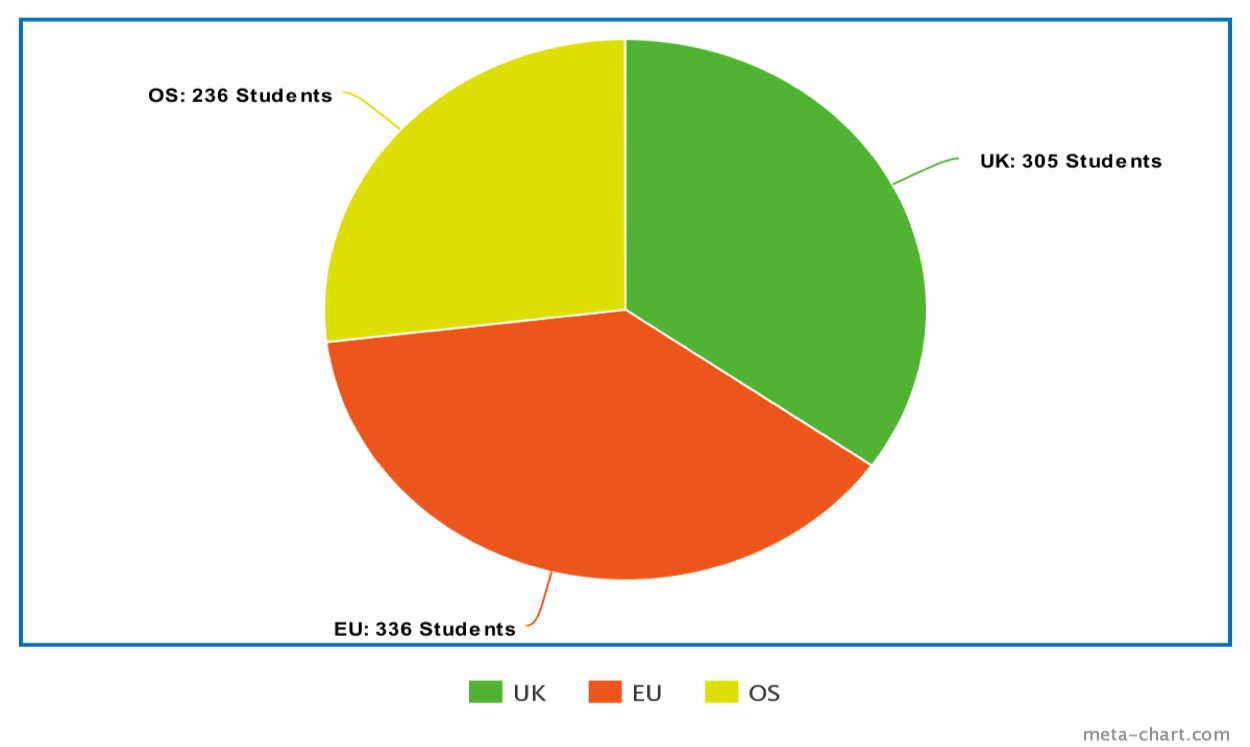
\includegraphics[width=1\linewidth]{images/ugstudentspiechart} 

}

\caption{Where our undergraduate students come from: As of October 2019 we have 877 undergraduate Computer Science students divided between UK/EU (shown in green), EU not UK (shown in orange) and non-EU overseas (shown in yellow)}\label{fig:pie-fig}
\end{figure}

\hypertarget{careersfairs}{%
\section{Careers fairs}\label{careersfairs}}

Our annual Computer Science careers fair is held in the Kilburn building in autumn, we typically have around 30 employers exhibiting over two days. As space is limited, we are always over-subscribed and are not able to accommodate every employer that our students will be interested in. We give priority to employers that offer internships, placements and graduate roles and have contributed to our community through the activities described on this page. The central careers service also organises:

\begin{itemize}
\tightlist
\item
  the big careers fair in \href{https://www.manchestercentral.co.uk/}{Manchester Central} every autumn, see the \href{http://www.careers.manchester.ac.uk/events/bigcareersfair/}{Big Careers Fair}
\item
  a smaller careers fair in Fallowfield \href{http://www.sport.manchester.ac.uk/facilities/armitage/}{Armitage centre} in May
\item
  hundreds of other employer events on campus during term time \citep{highfliers2020}
\end{itemize}

\hypertarget{dropins}{%
\section{Drop-in sessions}\label{dropins}}

If you aren't willing or able to exhibit at careers fairs, we also run ad-hoc drop-in sessions where employers can come in and set up a stand in the foyer to talk to computer science students informally on their way to and from lectures. These usually happen during lunch in \href{https://www.manchester.ac.uk/discover/key-dates/}{term time}. If you're interested in exhibiting at either of these events, please \protect\hyperlink{Contact}{contact the careers and placements officer Mabel Yau}.

\hypertarget{industryclub}{%
\section{Industry Club}\label{industryclub}}

\begin{center}
\includegraphics[width=0.4\linewidth]{images/industry-club-black} \end{center}

All employers are welcome to join our industry club mailing list by sending an email to \href{mailto:listserv@listserv.manchester.ac.uk}{\nolinkurl{listserv@listserv.manchester.ac.uk}} with the the text \textbf{subscribe cs-industryclub yourfirstname yoursecondname} in the body of the email message. The industry club is part of our \href{https://www.cs.manchester.ac.uk/connect/business-engagement/}{wider business engagement activities}.

The mailing list is low-traffic, typically two to three updates per year and an invitation to our annual industry club meeting. We promise not to spam you or sell your email details on to third parties.

\hypertarget{mentoring}{%
\section{Industrial mentoring}\label{mentoring}}

The \href{https://www.cs.manchester.ac.uk/connect/business-engagement/industrial-mentoring/}{Industrial mentoring scheme for software engineers} allows employers meet students during code review sessions.

\hypertarget{cosupervise}{%
\section{Co-supervised projects}\label{cosupervise}}

If you would like to co-supervise a project student in collaboration with an academic member of staff, there are several options. The best option depends on the domain, level and duration of the project:

\begin{itemize}
\tightlist
\item
  \textbf{Bachelors projects}: these are completed in the final year of a Bachelors degree and last for six months, starting in September and finishing in March. Projects are proposed (and offered to students) in March and start in September of the same year.
\item
  \textbf{Masters projects}: again these are six months in duration but start in March and finish in September. Projects are proposed (and offered to students) in the preceding November.
\item
  \textbf{PhD projects}: For industrially sponsored or co-supervised projects, speak to the research office at \href{https://www.cs.manchester.ac.uk/research/}{cs.manchester.ac.uk/research}.
\item
  \textbf{Knowledge Transfer Partnerships}: We have a range of \href{https://www.gov.uk/guidance/knowledge-transfer-partnerships-what-they-are-and-how-to-apply}{KTPs}, speak to the research office for details
\item
  \textbf{Impact Acceleration Accounts}: We have a range of \href{https://epsrc.ukri.org/innovation/fundingforimpact/impact-acceleration-accounts/}{IAAs}, speak to the research office for details
\end{itemize}

For Bachelors and Masters projects, you can contact academic members of staff directly, or speak to \href{https://www.research.manchester.ac.uk/portal/tim.morris.html}{Tim Morris} (final year project lead) or \href{https://www.research.manchester.ac.uk/portal/caroline.jay.html}{Caroline Jay}, who leads our postgraduate taught (Masters) courses.

\hypertarget{the-wednesday-waggle}{%
\section{The Wednesday Waggle}\label{the-wednesday-waggle}}

During term time, we highlight events and vacancies for Computer Science students from a \href{http://dullhunk.github.io/where-can-I-look-for-jobs.html}{wide range of sources} in a weekly newsletter called the \href{https://waggle.cs.manchester.ac.uk/waggle/about}{Wednesday Waggle} 🐝. This goes out to around \textasciitilde1000 Bachelors and Masters students in Manchester each week. If you have vacancies or events you would like our students to know about, \protect\hyperlink{contact}{get in touch with us} or \href{http://www.careers.manchester.ac.uk/aboutus/contact/}{contact the careers service}.

\hypertarget{join-the-community}{%
\section{Join the community}\label{join-the-community}}

There is a thriving community of engineers and \href{https://www.manchesterentrepreneurs.co.uk/}{entrepreneurs} in Manchester and across the North of England. One of the best ways to recruit engineers and scientists is to join and \emph{contribute} to the community. Get involved in events, \href{https://www.unicsmcr.com/}{sponsor a hackathon}, deliver a guest lecture, host your own event or \href{https://www.cs.manchester.ac.uk/connect/business-engagement/industrial-mentoring/}{become a software engineering mentor}. Employers who engage \textbf{early and often} are much more likely to get something back. As an employer, you may also be interested in events run by:

\begin{itemize}
\tightlist
\item
  The \href{https://ise.org.uk}{Institute of Student Employers} (ISE)
\item
  The \href{https://www.agcas.org.uk}{Association of Graduate Careers Advisory Services} (AGCAS)
\item
  The \href{https://www.asetonline.org}{Work Based and Placement Learning Association} (ASET)
\end{itemize}

If you're a startup new to employment, you may find the guide at \href{https://www.gov.uk/employ-someone}{gov.uk/employ-someone} useful.

\hypertarget{buzzing}{%
\section{Buzzing!}\label{buzzing}}

At peak times, we can get \textbf{very busy} with many concurrent employer events on campus. \citep{highfliers2020} Please be patient and persistent if we do not reply immediately. Unfortunately, we are not always able to respond to everyone because our students, staff and space are all finite resources. We give priority to employers that have already given their time and expertise to our community.



\begin{figure}

{\centering 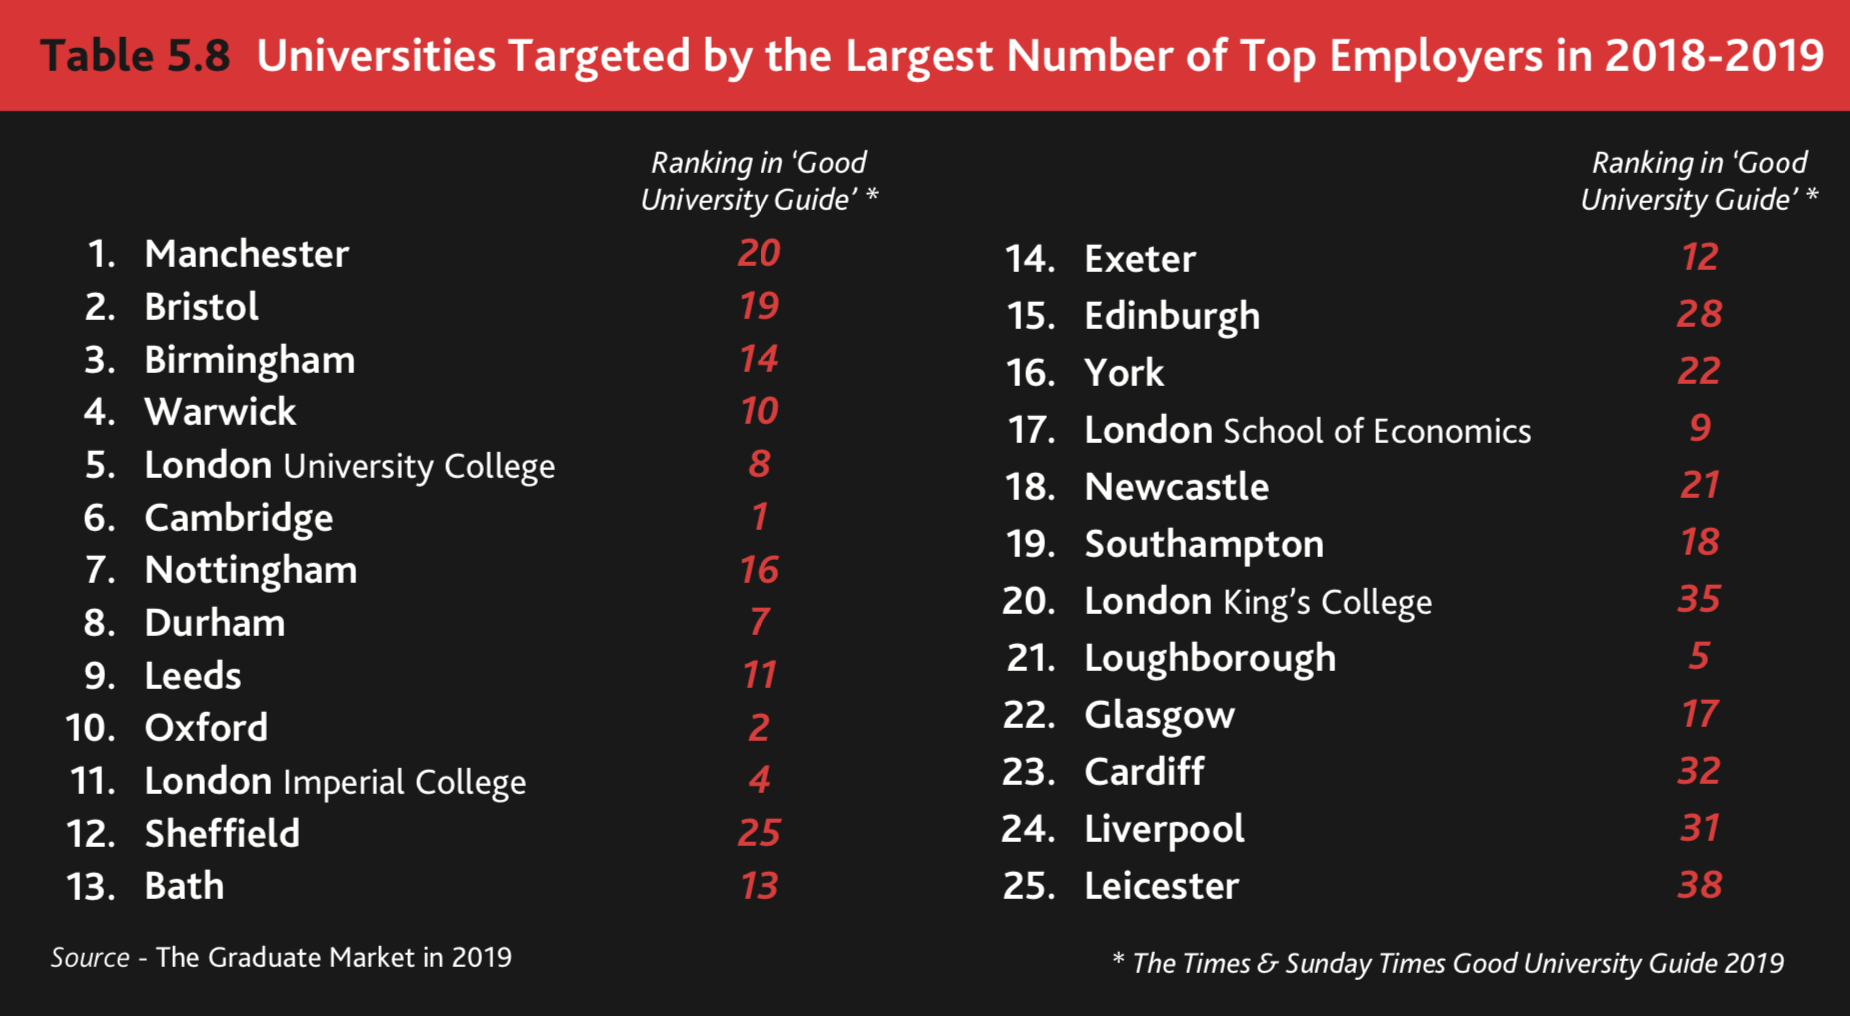
\includegraphics[width=1\linewidth]{images/high-fliers-table} 

}

\caption{According to \href{https://www.highfliers.co.uk}{highfliers.co.uk}, the University of Manchester is the most targeted University in the UK by the \href{https://www.top100graduateemployers.com}{Times Top 100 Graduate Employers} \citep{highfliers2020}}\label{fig:unnamed-chunk-4}
\end{figure}

\hypertarget{employability}{%
\section{Employability}\label{employability}}

We are working hard to improve the employability of students because while having a Computer Science is necessary for some jobs, it is not sufficient. \citep{unemployed, shadboltreview, fincherreview, finchergecco} Over the last decade we have been successful in \emph{more than doubling} the number of our students going on year long placements in industry. This is a win-win-win situtation for:

\begin{enumerate}
\def\labelenumi{\arabic{enumi}.}
\tightlist
\item
  \textbf{Students}: benefit from a broader education, and develop social and non-cognitive skills that can be challenging to teach and learn in a purely academic environment. This is known as the \href{https://www.suttontrust.com/research-paper/a-winning-personality-confidence-aspirations-social-mobility/}{winning personality} \citep{winningpersonality}.
\item
  \textbf{Employers}: placements are a cost-effective way for employers to recruit (and retain) graduate talent
\item
  \textbf{Universities}: produce better graduates \citep{Mandilaras2004} with broader and deeper skills, who earn more and get better jobs \citep{winningpersonality}. Well paid placements can also facilitate social mobility. \citep{Wang2018}
\end{enumerate}

\begin{longtable}[]{@{}ll@{}}
\toprule
\begin{minipage}[b]{(\columnwidth - 1\tabcolsep) * \real{0.50}}\raggedright
year placement started\strut
\end{minipage} & \begin{minipage}[b]{(\columnwidth - 1\tabcolsep) * \real{0.50}}\raggedright
No.~of Computer Science undergraduate students on placement\strut
\end{minipage}\tabularnewline
\midrule
\endhead
\begin{minipage}[t]{(\columnwidth - 1\tabcolsep) * \real{0.50}}\raggedright
2008\strut
\end{minipage} & \begin{minipage}[t]{(\columnwidth - 1\tabcolsep) * \real{0.50}}\raggedright
35\strut
\end{minipage}\tabularnewline
\begin{minipage}[t]{(\columnwidth - 1\tabcolsep) * \real{0.50}}\raggedright
2009\strut
\end{minipage} & \begin{minipage}[t]{(\columnwidth - 1\tabcolsep) * \real{0.50}}\raggedright
31\strut
\end{minipage}\tabularnewline
\begin{minipage}[t]{(\columnwidth - 1\tabcolsep) * \real{0.50}}\raggedright
2010\strut
\end{minipage} & \begin{minipage}[t]{(\columnwidth - 1\tabcolsep) * \real{0.50}}\raggedright
45\strut
\end{minipage}\tabularnewline
\begin{minipage}[t]{(\columnwidth - 1\tabcolsep) * \real{0.50}}\raggedright
2011\strut
\end{minipage} & \begin{minipage}[t]{(\columnwidth - 1\tabcolsep) * \real{0.50}}\raggedright
42\strut
\end{minipage}\tabularnewline
\begin{minipage}[t]{(\columnwidth - 1\tabcolsep) * \real{0.50}}\raggedright
2012\strut
\end{minipage} & \begin{minipage}[t]{(\columnwidth - 1\tabcolsep) * \real{0.50}}\raggedright
45\strut
\end{minipage}\tabularnewline
\begin{minipage}[t]{(\columnwidth - 1\tabcolsep) * \real{0.50}}\raggedright
2013\strut
\end{minipage} & \begin{minipage}[t]{(\columnwidth - 1\tabcolsep) * \real{0.50}}\raggedright
70\strut
\end{minipage}\tabularnewline
\begin{minipage}[t]{(\columnwidth - 1\tabcolsep) * \real{0.50}}\raggedright
2014\strut
\end{minipage} & \begin{minipage}[t]{(\columnwidth - 1\tabcolsep) * \real{0.50}}\raggedright
54\strut
\end{minipage}\tabularnewline
\begin{minipage}[t]{(\columnwidth - 1\tabcolsep) * \real{0.50}}\raggedright
2015\strut
\end{minipage} & \begin{minipage}[t]{(\columnwidth - 1\tabcolsep) * \real{0.50}}\raggedright
70\strut
\end{minipage}\tabularnewline
\begin{minipage}[t]{(\columnwidth - 1\tabcolsep) * \real{0.50}}\raggedright
2016\strut
\end{minipage} & \begin{minipage}[t]{(\columnwidth - 1\tabcolsep) * \real{0.50}}\raggedright
65\strut
\end{minipage}\tabularnewline
\begin{minipage}[t]{(\columnwidth - 1\tabcolsep) * \real{0.50}}\raggedright
2017\strut
\end{minipage} & \begin{minipage}[t]{(\columnwidth - 1\tabcolsep) * \real{0.50}}\raggedright
100\strut
\end{minipage}\tabularnewline
\begin{minipage}[t]{(\columnwidth - 1\tabcolsep) * \real{0.50}}\raggedright
2018\strut
\end{minipage} & \begin{minipage}[t]{(\columnwidth - 1\tabcolsep) * \real{0.50}}\raggedright
97\strut
\end{minipage}\tabularnewline
\begin{minipage}[t]{(\columnwidth - 1\tabcolsep) * \real{0.50}}\raggedright
2019\strut
\end{minipage} & \begin{minipage}[t]{(\columnwidth - 1\tabcolsep) * \real{0.50}}\raggedright
110\strut
\end{minipage}\tabularnewline
\bottomrule
\end{longtable}

In 2019 our students have secured year long placements at Accenture, Agilent Technologies, Amazon (2), AND Digital, Apadmi (5), Arggo, ARM (5), Autodesk, AVL Powertrain, BAML, the BBC (2), Biorelate, BJSS, Bloomberg (2), BMW Mini, Bsquare Controls (2), BT, Cantarus (3), Celtra, CERN (3), Codethink, d3t, Elysian Systems, Feral Interactive (2), Fidelity, FiveAI, HMRC, IBM (2), Imagination Technologies, Intel (4), ISA Software (2), JP Morgan (4), Keysight Technologies, KPMG (1), Matillion (4), McAfee (2), Mentor Graphics (4), Monoprix, Morgan Stanley (2), NCC Group, Nokia, Nomura, Novacoast (2), Ocado (3), PA Consulting, PwC, Schlumberger, ServiceNow, Siemens (3), Soda Software, SteamaCo, The Hut Group (10),
The Start Up Factory (2), Uber, Visa and Vodafone.

There's still more we can do to improve the employability of our graduates. If you'd like to help our graduates become more employable, \href{Contact}{get in touch}.

\hypertarget{research}{%
\chapter{Research}\label{research}}

My research interests are in \href{https://en.wikipedia.org/wiki/Computer_science_education}{Computer Science Education} and \href{https://en.wikipedia.org/wiki/Pedagogy}{pedagogy}. \citep{CERhandbook, JohnBiggs2011, Fry2014} I'm interested in methods that can improve learning and student experience using techniques like \href{https://www.cdyf.me}{coding your future}, \href{https://sigcse.cs.manchester.ac.uk/}{journal clubbing}, \href{https://www.cs.manchester.ac.uk/connect/business-engagement/industrial-mentoring/}{industrial mentoring}, \protect\hyperlink{tuningcomplete}{live music}, \href{http://www.cs.man.ac.uk/~hulld/coding-their-future.html}{working with schools}, \href{http://www.cs.man.ac.uk/~hulld/vertical-tutoring.html}{vertical tutoring}, \protect\hyperlink{wikipedia}{editing Wikipedia} and more.

\begin{figure}

{\centering 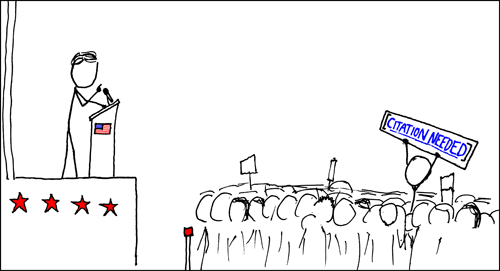
\includegraphics[width=0.7\linewidth]{images/wikipedian_protester} 

}

\caption{Too many educational practices are not backed up by good evidence that they actually work. More evidence is needed to support many of the claims made about effective pedagogy. \emph{Wikipedian Protester} cartoon by \href{https://en.wikipedia.org/wiki/Randall_Munroe}{Randall Munroe} at \href{https://xkcd.com/285/}{xkcd.com/285} published under a \href{https://creativecommons.org/licenses/by-nc/2.5/}{Creative Commons Attribution-NonCommercial 2.5 License}}\label{fig:unnamed-chunk-5}
\end{figure}



\hypertarget{sigcse}{%
\section{SIGCSE}\label{sigcse}}

Computer Science has only been taught to undergraduates in the UK for 50 short years \citep{babygrowsup, sigcse50}, so there's lots of open questions about how to teach the practical, theoretical and professional aspects of the subject. To that end:

\begin{itemize}
\tightlist
\item
  I'm an \href{https://dl.acm.org/profile/81350580198}{active member} of the \href{https://en.wikipedia.org/wiki/Association_for_Computing_Machinery}{Association for Computing Machinery} (ACM) and it's Special Interest Group (SIG) in Computer Science Education (\href{https://sigcse.org}{sigcse.org}). In 2020 I founded the \href{https://sigcse.cs.manchester.ac.uk/}{ACM SIGCSE journal club} and chair the monthly Manchester meetup. Anyone is welcome to join, see \href{https://sigcse.cs.manchester.ac.uk/join-us}{sigcse.cs.manchester.ac.uk/join-us}
\item
  I serve on the program committee of the \href{https://www.ukicer.com/}{United Kingdom and Ireland Computing Education Research (UIKICER)} conference, on the board of \href{https://uki-sigcse.acm.org/about}{UK ACM SIGCSE} and have served on the program committee for \href{http://community.dur.ac.uk/cep.conference}{Computing Education \& Practice (CEP)} conference at Durham University
\end{itemize}

\hypertarget{industrial-mentoring}{%
\section{Industrial mentoring}\label{industrial-mentoring}}

Since we started the \href{https://www.cs.manchester.ac.uk/connect/business-engagement/industrial-mentoring/}{Industrial mentoring scheme for software engineers} in 2015, more than 1000 students have been through the mentoring scheme with 250 students taking the course every year. We are very grateful for continued support from our industrial partners in making this happen.

Mentors meet with a group of six second year students for two one hour meetings and do some gentle code review of their gitlab repository, as they start to fix bugs and add features to a large open source software project. You don't \emph{need} to be an expert in the tools students are using (Java, Eclipse, Jenkins, Git, JUnit and Ant) it is more about the general process (and politics) of building and testing high quality software in large and distributed teams, than the specifics of the codebase (\url{https://stendhalgame.org/}) we happen to be using. Mentors are typically software engineers, both junior and senior.

\hypertarget{vt}{%
\section{Vertical tutoring}\label{vt}}

We are currently piloting a vertical tutoring (VT) scheme, see \href{http://www.cs.man.ac.uk/~hulld/vertical-tutoring.html}{vertical tutoring} for details. \citep{vtbernard, druryvert}

\hypertarget{codeclub}{%
\section{Coderdojo \& Code Club}\label{codeclub}}

I'm a volunteer at \href{https://coderdojo.com/}{coderdojo.com} \citep{coderdojo}. Coder \href{https://en.wikipedia.org/wiki/Dojo}{dojos} are local community engineering clubs for young people; with several other volunteers I help out at \href{https://twitter.com/coderdojonw}{CoderDojo North West}. We meet once a month to help young people broaden their digital and computational horizons.

Previously I lead an after school \href{https://codeclub.org}{CodeClub} as part of a global network of free coding clubs for 9--13 year olds. \citep{codeclub} As with coderdojo, the aim is to have fun using \href{https://scratch.mit.edu/}{Scratch}, \citep{Resnick2009} python and other interesting technology we can get our hands on including \href{https://www.raspberrypi.org/}{Raspberry Pi}, \citep{raspberrypi} \href{https://microbit.org/}{Micro:bits}, \citep{Sentance2017} \href{https://www.lego.com/en-gb/themes/mindstorms}{LEGO® MINDSTORMS®}, \citep{Papert1980, Klassner2003} \href{https://www.oculus.com}{Oculus Rift}, \href{https://sonic-pi.net/}{Sonic Pi} \citep{Aaron2016} and \href{http://www.codebug.org.uk/}{CodeBug} etc.

\hypertarget{wikipedia}{%
\section{Wikipedia}\label{wikipedia}}

Wikipedia and \href{https://www.wikidata.org}{wikidata.org} \citep{Vrandecic2014, Turki2019} are powerful tools for improving both digital skills and communication skills, regardless of your age or level of computer literacy, \citep{Proffitt2018, goodfaith, Littlejohn2019} particularly in the following areas:

\begin{itemize}
\tightlist
\item
  \href{https://en.wikipedia.org/wiki/Literacy}{Literacy} generally, the ability to read and write in any natural language. The literacy skills of some engineers and scientists leaves plenty of room for improvement, but literacy has many overlapping dimensions including:

  \begin{itemize}
  \tightlist
  \item
    \href{https://en.wikipedia.org/wiki/Data_literacy}{Data literacy} the ability to read and write (data)
  \item
    \href{https://en.wikipedia.org/wiki/Digital_literacy}{Digital literacy} the ability to read and write (digitally)
  \item
    \href{https://en.wikipedia.org/wiki/Computer_literacy}{Computer literacy} the ability to read and write (using a computer)
  \item
    \href{https://en.wikipedia.org/wiki/Information_literacy}{Information literacy} the ability to read and write (information)
  \item
    \href{https://en.wikipedia.org/wiki/Scientific_literacy}{Scientific literacy} the ability to read and write (science). How many people do you know who \emph{unashamedly} proclaim their scientific or mathematical illiteracy? \citep{nevergoodatmaths, gowersproblem, mathillit}
  \end{itemize}
\end{itemize}

As an experienced and long serving editor of Wikipedia since 2004, I organise and participate in \href{https://en.wikipedia.org/wiki/Edit-a-thon}{Wikipedia training events} which recruit new Wikipedia editors. Some recent examples include:

\begin{enumerate}
\def\labelenumi{\arabic{enumi}.}
\tightlist
\item
  2020-06-24 \href{https://en.wikipedia.org/wiki/Wikipedia:Meetup/Women_in_War_and_Peace}{Wikipedia: Women, War and Peace} run in collaboration with the \href{https://www.iwm.org.uk/partnerships/subject-specialist-network}{Imperial War Museums' War and Conflict Subject Specialist Network}, with support from the Arts Council England and Art Fund.
\item
  2020-02-26 \href{https://wikiedusummit.coventry.domains}{Wikimedia in Education UK Summit, Coventry University} \#wikiedu20
\item
  2019-11-22 \href{https://duncan.hull.name/2019/12/10/glasgow/}{Training of Trainers (ToT) workshop, University of Glasgow}
\item
  2019-10-19 \href{https://wiki-loves-scientists.org.uk/2019/10/09/learn-to-edit-wikipedia-thurs-17th-october-university-of-manchester-all-welcome/}{Learn to edit Wikipedia with Ada Lovelace}, \href{https://en.wikipedia.org/wiki/Sackville_Street_Building}{Sackville Street Building}, University of Manchester \citep{findingada2019}
\item
  2019-10-12 \href{https://www.eventbrite.com/e/global-wikipedia-edit-a-thon-wikieditathon-2019-manchester-and-london-2019-zebra-hub-hq-the-tickets-48601581639}{Wikipedia Edit-a-Thon with Zebra Hub HQ}, \href{https://en.wikipedia.org/wiki/Pankhurst_Centre}{Pankhurst Centre}, Manchester
\item
  2017-10-13 \href{https://wiki-loves-scientists.org.uk/2017/10/27/mirror-mirror-on-the-wall-who-is-the-most-viewed-of-them-all/}{Physiology Friday, Hodgkin Huxley House}, Farringdon, London \citep{goodbadugly}
\item
  2015-09-02 \href{https://wikimedia.org.uk/wiki/Wikipedia_Science_Conference}{First Wikipedia Science Conference \#wikisci}, \href{https://en.wikipedia.org/wiki/Wellcome_Collection}{Wellcome Collection}, London, NW1 \citep{troubled, Hodson2015}
\end{enumerate}

More information on past and future events like this can be found at:

\begin{itemize}
\tightlist
\item
  \href{https://wiki-loves-scientists.org.uk/}{wiki-loves-scientists.org.uk}
\item
  \href{https://en.wikipedia.org/wiki/User:Duncan.Hull}{en.wikipedia.org/wiki/User:Duncan.Hull}
\end{itemize}

\hypertarget{tuningcomplete}{%
\section{Tuning complete}\label{tuningcomplete}}

Tuning complete are a \href{https://en.wikipedia.org/wiki/Musical_collective}{musical collective} from \href{https://duncan.hull.name/2019/07/05/mancashire/}{Manchester, Lancashire 🌹}, named after the famous Computer Scientist \href{https://en.wikipedia.org/wiki/Alan_Turing}{Alan Tuning}. We use his eponymous \href{https://en.wikipedia.org/wiki/Turing_machine}{Tuning machine} to make music which is quality assured using the \href{https://en.wikipedia.org/wiki/Turing_test}{Tuning test}. As of 2020, our lineup includes the following artists:

\begin{itemize}
\tightlist
\item
  \href{https://www.linkedin.com/in/jez-lloyd-84077069}{Jez Lloyd}: Bachelor of Music, DJ and backing vocals
\item
  \href{https://en.wikipedia.org/wiki/Steve_Furber}{Steve Furber}: six string guitar and bass
\item
  \href{https://en.wikipedia.org/wiki/Justin_Timberlake}{Justin Timberfake}: lead vocals, lead dancer
\item
  \href{https://en.wikipedia.org/wiki/Billie_Eilish}{Billie Fakish}: guest vocalist
\item
  Duncan Hull: MC, synth (\href{https://en.wikipedia.org/wiki/MicroKORG}{MicroKORG}), drum machine (\href{https://sonic-pi.net/}{Sonic Pi}) and embarrassing dad dancing \citep{daddancing}
\end{itemize}

Theoretically, we are a \href{https://en.wikipedia.org/wiki/Turing_completeness}{Turing Complete} band. \citep{Turing1937, turingcomplete} Artistically, this means that what we lack in youth, good looks, fame, fortune, fashion sense, fanbase and back catalogue we compensate for with:

🤓 Musical geekery \citep{musicnmaths, behindthemusic}\\
🤓 Mathematical geekery \citep{plusmaths}\\
🤓 Computer geekery \citep{Aaron2016}

\begin{figure}

{\centering 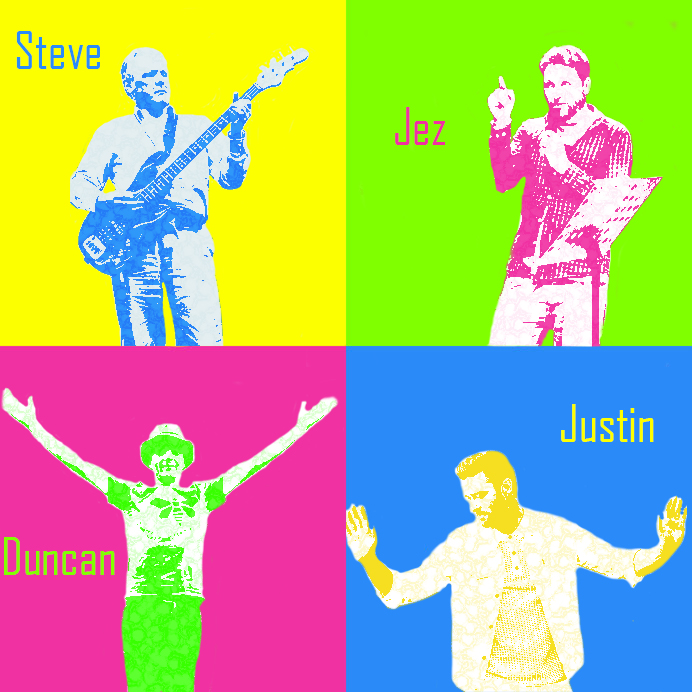
\includegraphics[width=0.7\linewidth]{images/tuning-complete} 

}

\caption{Tuning Complete consists of Jez Lloyd, Steve Furber, Justin Timberfake and me.}\label{fig:beatles-fig}
\end{figure}

We played our debut gigs to packed theatres of over 200 second year \& first year undergraduate computer science students in the autumn of 2019 and are currently planning future live events while writing a (hopefully) lucrative hit single, working title: \href{https://twitter.com/hashtag/LivingTheDream}{\#LivingTheDream}. If you would like to book our services for your next event, hackathon, wedding, bar mitzvah etc, please contact our agent Mrs.~Kilburn shown in Figure \ref{fig:mrskilburn-fig}.

\begin{figure}

{\centering 
\includegraphics[width=0.7\linewidth]{images/mrs-kilburn} 

}

\caption{Mrs. Kilburn is our manager, booking agent and promoter. She is the power behind our boy band throne, so all bookings must be approved and scheduled by her office. Please do not approach band members directly with gig requests or offers of marriage, we are all answered for!}\label{fig:mrskilburn-fig}
\end{figure}

\hypertarget{publications}{%
\section{Publications}\label{publications}}

Informal publications can be found on my sporadically updated blog

\begin{itemize}
\tightlist
\item
  \href{https://duncan.hull.name/lablog/}{duncan.hull.name/lablog}
\end{itemize}

Formal peer-reviewed publications can be found on DBLP, ORCID, Google Scholar, the ACM Digital Library, Wikidata etc:

\begin{itemize}
\tightlist
\item
  \href{https://dblp.org/pid/h/DuncanHull}{dblp.org/pid/h/DuncanHull}
\item
  \href{https://www.wikidata.org/wiki/Q47012855}{wikidata.org/wiki/Q47012855}
\item
  \href{https://orcid.org/0000-0003-2387-503X}{orcid.org/0000-0003-2387-503X}
\item
  \href{https://dl.acm.org/profile/81350580198}{dl.acm.org/profile/81350580198}
\item
  \href{https://scholar.google.com/citations?user=iDJ-t7IAAAAJ}{scholar.google.com/citations?user=iDJ-t7IAAAAJ}
\end{itemize}

According to Google scholar, my most cited papers are on:

\begin{enumerate}
\def\labelenumi{\arabic{enumi}.}
\tightlist
\item
  Apache Taverna, published in \href{https://en.wikipedia.org/wiki/Nucleic_Acids_Research}{\emph{Nucleic Acids Research}} \citep{taverna}\\
\item
  Another Taverna paper, published in \emph{Concurrency and Computation} \citep{Oinn2006}\\
\item
  A paper on modelling human metabolism, published in \href{https://en.wikipedia.org/wiki/Nature_Biotechnology}{\emph{Nature Biotechnology}} \citep{Thiele2013}
\item
  A review of tools for managing large bibliographies, published in \href{https://en.wikipedia.org/wiki/PLOS_Computational_Biology}{\emph{PLOS Computational Biology}} \citep{defrosting}
\end{enumerate}

The first paper for which I was formally acknowledged was on simulated environmental change in the sub-arctic published in \href{https://en.wikipedia.org/wiki/New_Phytologist}{\emph{New Phytologist}} \citep{subarctic}. I was a humble field assistant, not a co-author, one of the \emph{absolut} best summer jobs I've ever had!

\hypertarget{vertical-tutoring}{%
\chapter{Vertical tutoring}\label{vertical-tutoring}}

We are currently piloting a vertical tutoring (VT) system for undergraduate students. VT is already widespread in secondary education, \citep{vtbernard, druryvert} but as far as we know has not been widely used in higher education.

Extending the idea of Peer Assisted Study Sessions (PASS) \href{http://www.pass.manchester.ac.uk}{pass.manchester.ac.uk}, \citep{passeffect} vertical tutoring creates tutorial groups with a representative from \emph{one of each} year of undergraduate study combined with alumni.

\begin{figure}

{\centering 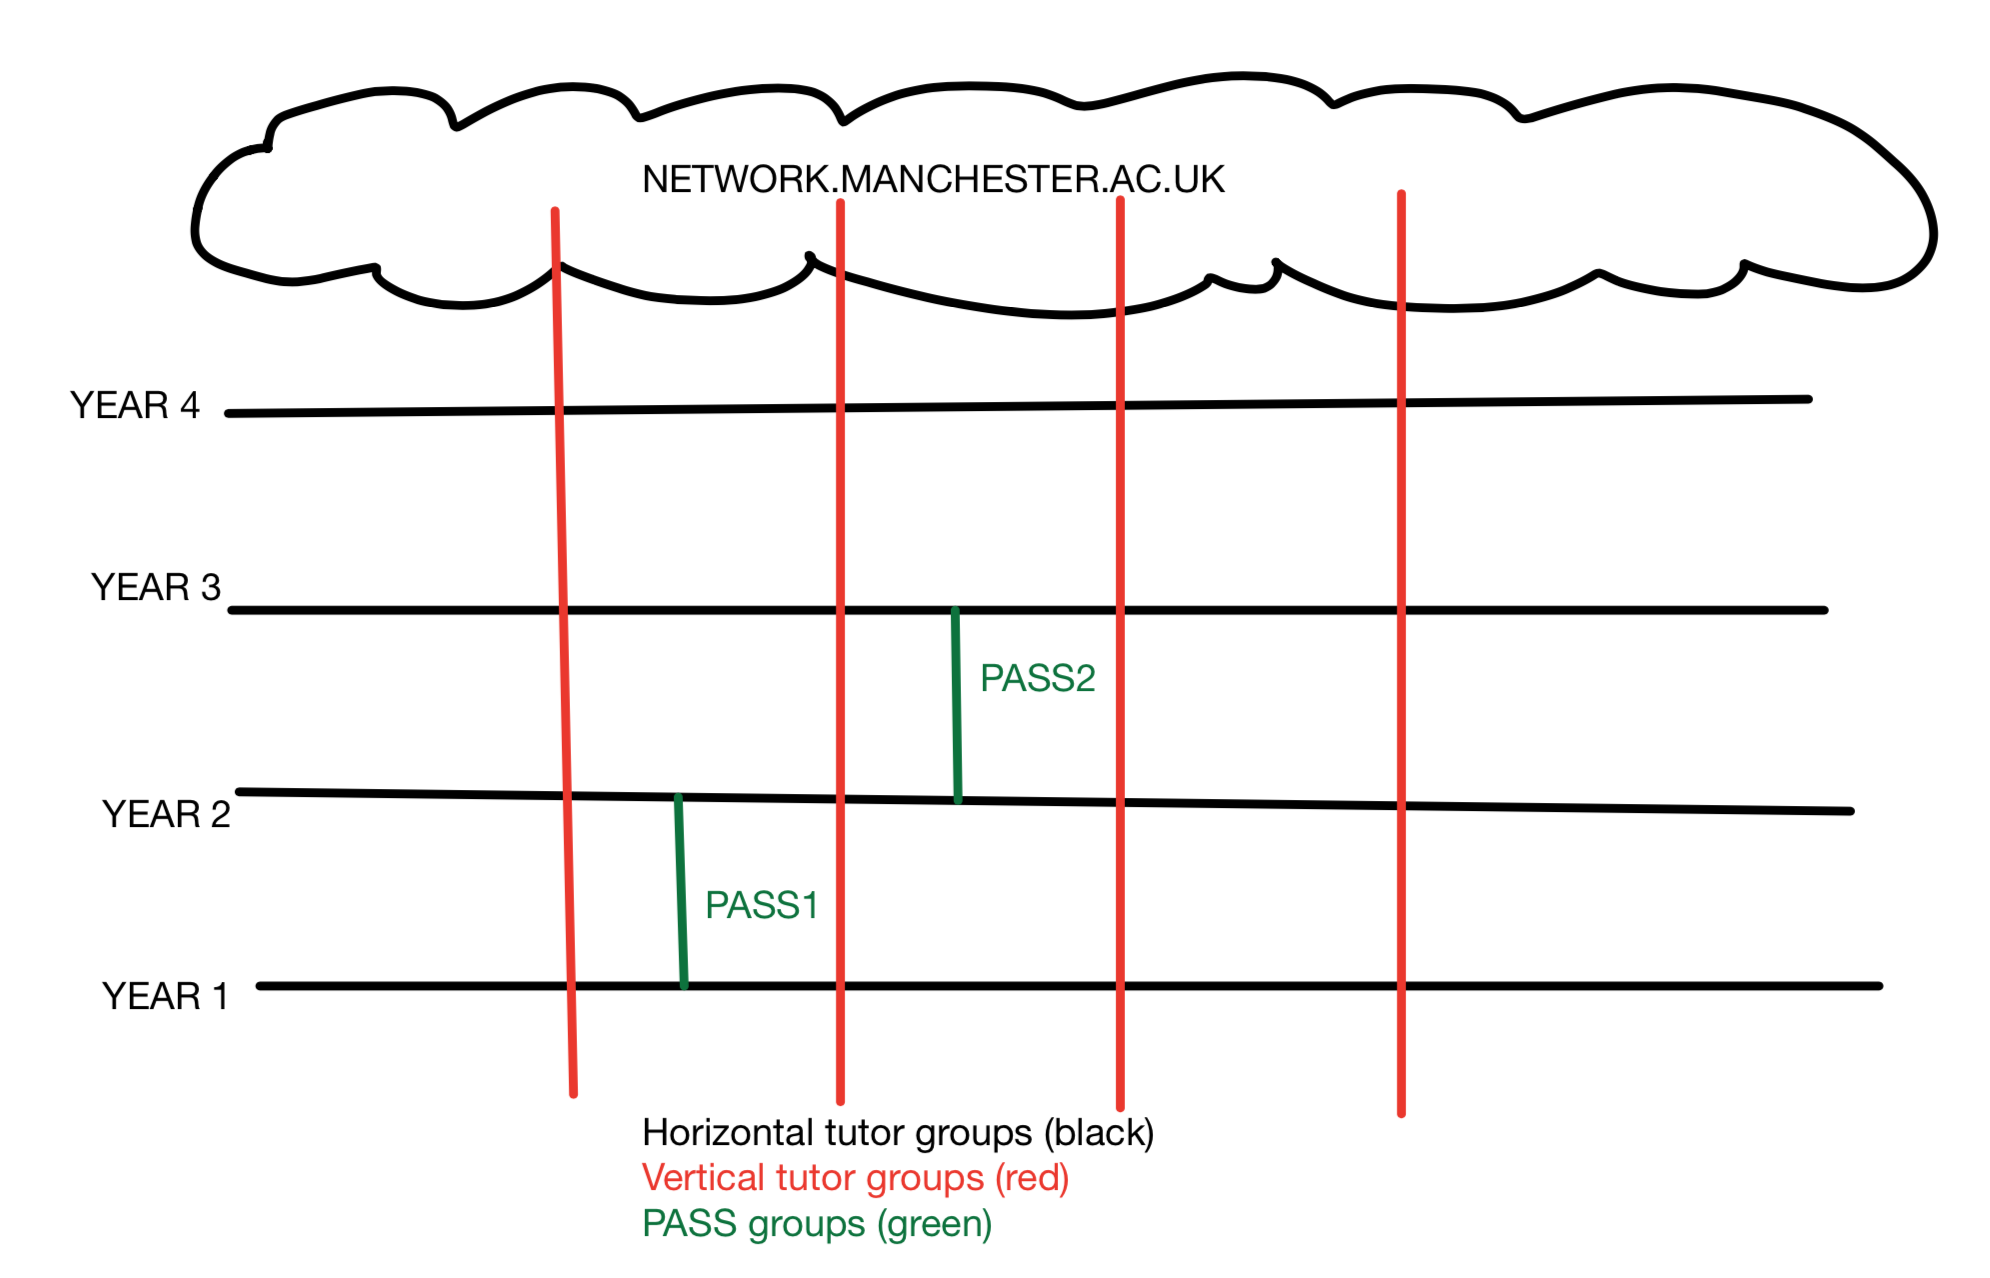
\includegraphics[width=1\linewidth]{images/vertical-tutor-groups} 

}

\caption{Conventional horizontal tutor groups (shown in black) bring together a group of students in the same year. For example, year 1 students meet as a small group once per week during term time with their tutor. Vertical tutor groups (shown in red) are made of of one student from each year and an alumni. Vertical tutor groups extend the idea of PASS, to full stack mentoring, crossing all levels}\label{fig:vertical-fig}
\end{figure}

\hypertarget{fullstack}{%
\section{Full stack mentoring}\label{fullstack}}

A vertical tutor group will typically contain five members as shown in Figure \ref{fig:vertical-fig}. The group meets physically where possible, or virtually via a slack channel which consists of:

\begin{enumerate}
\def\labelenumi{\arabic{enumi}.}
\tightlist
\item
  One first year student
\item
  One second year student
\item
  One penultimate year student (out on industrial placement)
\item
  One final year student (returned from placement or summer internship)
\item
  One member of our alumni, recent graduate or via \href{https://www.network.manchester.ac.uk/}{network.manchester.ac.uk}
\end{enumerate}

Vertical tutor groups meet twice per semester. It is very unlikely that a free timetable slot for all years and alumni can be found during normal office hours, because of the complexities of timetabling. So evenings will be likely to work best. Where possible, tutor groups will meet face to face, with remote members (e.g.~placement students and alumni) typically joining virtually by slack or similar.

\hypertarget{goodfor}{%
\section{What is it good for?}\label{goodfor}}

Vertical tutoring is an attractive idea but does it actually work? If so, how? What is it useful for? We would like to find out:

\begin{enumerate}
\def\labelenumi{\arabic{enumi}.}
\tightlist
\item
  If there is any appetite for vertical tutoring amongst students and alumni
\item
  How it could work e.g.~with \href{https://slack.com}{slack.com} or \href{https://discordapp.com/}{discord} etc?
\item
  How many times can/should vertical tutor groups meet? Twice per semester? More frequently? Less frequently?
\item
  What are suitable topics for discussion in a vertical tutorial? Careers, wellbeing, networking etc
\item
  What kind of specialist groups could be useful e.g.~all female groups, research focussed tutorial groups (with MSc \& PhD students), ordinary ``vanilla'' groups etc
\item
  How much can we breakdown entrenched year groups that persist throughout education \citep{kills1}
\item
  What might the benefits be? \citep{kills2}
\end{enumerate}

As this is an experiment, students have been selected on a voluntary basis. If you are a student or former student and would like to get involved, let me know.

\hypertarget{howlong}{%
\section{How long will all this take?}\label{howlong}}

We ask that vertical tutees commit to:

\begin{itemize}
\tightlist
\item
  two one hour sessions per semester
\item
  allowing time for setup and administration, slack channels, scheduling suitable times and dates with your group
\item
  Two hours of time for feedback and review after each semester, by email survey
\end{itemize}

\hypertarget{coding-their-future}{%
\chapter{Coding their future}\label{coding-their-future}}

Coding their future is a collaboration \& partnership between secondary schools and the \href{https://www.cs.manchester.ac.uk/}{Department of Computer Science} at the University of Manchester. Our aims are to:

\begin{itemize}
\tightlist
\item
  improve and support Computer Science education at key stages 3, 4 and 5. \citep{shutdownrestart, afterthereboot, cse, cambridgegcse}
\item
  \href{https://www.manchester.ac.uk/discover/social-responsibility/widening-participation/}{widen participation in higher education}, especially in under-represented groups. \citep{wideningparticipation, classceiling, nicebutdim, breakintoelite}
\item
  enable our undergraduate students to develop their leadership and communication skills
\end{itemize}



\begin{figure}

{\centering 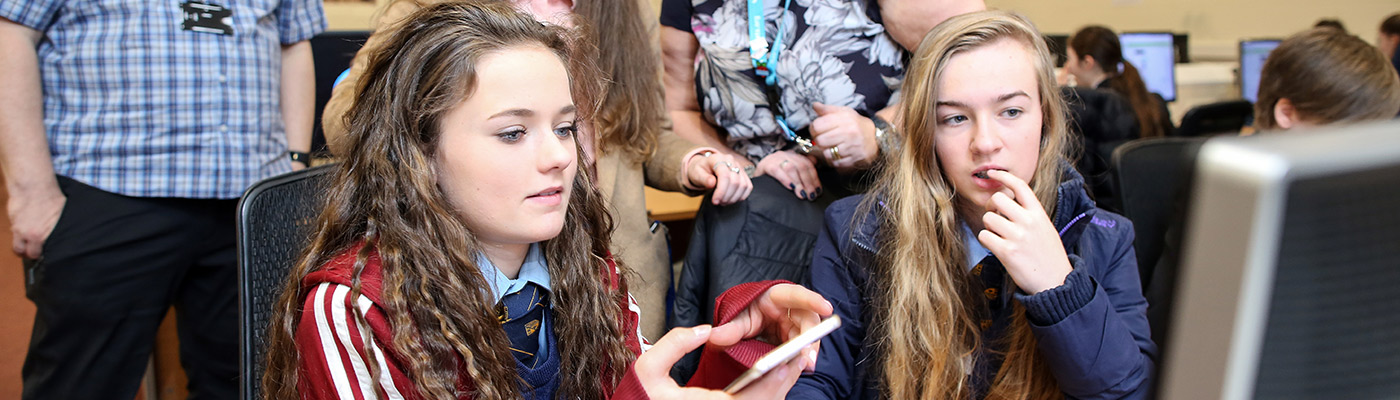
\includegraphics[width=1\linewidth]{images/schools-banner} 

}

\caption{Undergraduate students in computer science regularly work with schools as part of our wider \href{https://www.cs.manchester.ac.uk/connect/social-responsibility/}{social responsibility activities} \citep{m2020, m20202} and \href{https://www.cs.manchester.ac.uk/connect/schools-colleges-public/}{schools, colleges and public activities}}\label{fig:unnamed-chunk-6}
\end{figure}

The University provides schools with a final year student who can teach Computer Science in your school or college as a teaching assistant (TA). In return, the school provides our undergraduate students with a safe and supportive environment in which to teach which extends and augments your current curriculum. This can either be an after school, extension / lunchtime club or during scheduled lesson time, typically between year 7 and 13. This is similar to the \href{https://en.wikipedia.org/wiki/Undergraduate_Ambassadors_Scheme}{Undergraduate Ambassador Scheme} (UAS), \citep{uas, Cooper2005} and school placements \citep{Moller2019} except students work is assessed using our final year project framework. \citep{COMP30030, COMP30040} Since these projects were started in 2012, our students have worked with a range of schools in the private and public sector, both selective and non-selective, co-educational and single-sex including:

\begin{itemize}
\tightlist
\item
  \href{http://www.fairfieldhigh.tameside.sch.uk/}{Fairfield High School for Girls}, Droylsden
\item
  \href{https://www.trinityhigh.com}{Trinity CofE High School}, Central Manchester
\item
  \href{http://www.utcmediacityuk.org.uk/}{University Technical College (UTC) \(@\)MediaCityUK}, Salford
\item
  \href{https://www.manchestercommunicationacademy.com/}{Manchester Communication Academy}, Harpurhey\\
\item
  \href{https://thebarlowrchigh.co.uk/}{The Barlow RC High School}, Didsbury
\item
  \href{https://www.whgs-academy.org/}{William Hulme Grammar School}, Whalley Range
\item
  \href{https://www.chhs.org.uk/}{Cheadle Hulme High School}, (CHHS) Stockport
\item
  \href{https://www.lauruscheadlehulme.org.uk/}{Laurus Cheadle Hulme}, Stockport
\item
  \href{https://www.knutsfordacademy.org.uk/}{Knutsford Academy}, Knutsford
\item
  \href{http://www.aggs.trafford.sch.uk/}{Altrincham Grammar School for Girls}, Trafford
\item
  \href{https://www.agsb.co.uk/}{Altrincham Grammar School for Boys}, Trafford
\item
  \href{https://www.mgs.org/}{Manchester Grammar School} (MGS), Fallowfield
\end{itemize}

The projects were setup by \protect\hyperlink{contact}{Duncan Hull} and \href{http://www.cs.man.ac.uk/~david/}{David Rydeheard} (who retired in 2019), and are now run and supervised by Duncan. We hope to transfer ideas between private and public sector, as there are lots of open questions about how Computer Science should be taught. \citep{cse, suemcr, stephenson, fincherpetre} To find out more, see the \protect\hyperlink{guidance-for-teachers}{guidance for teachers} and \protect\hyperlink{guidance-for-students}{guidance for students} below.

\hypertarget{guidance-for-teachers}{%
\section{Guidance for teachers}\label{guidance-for-teachers}}



\begin{figure}

{\centering 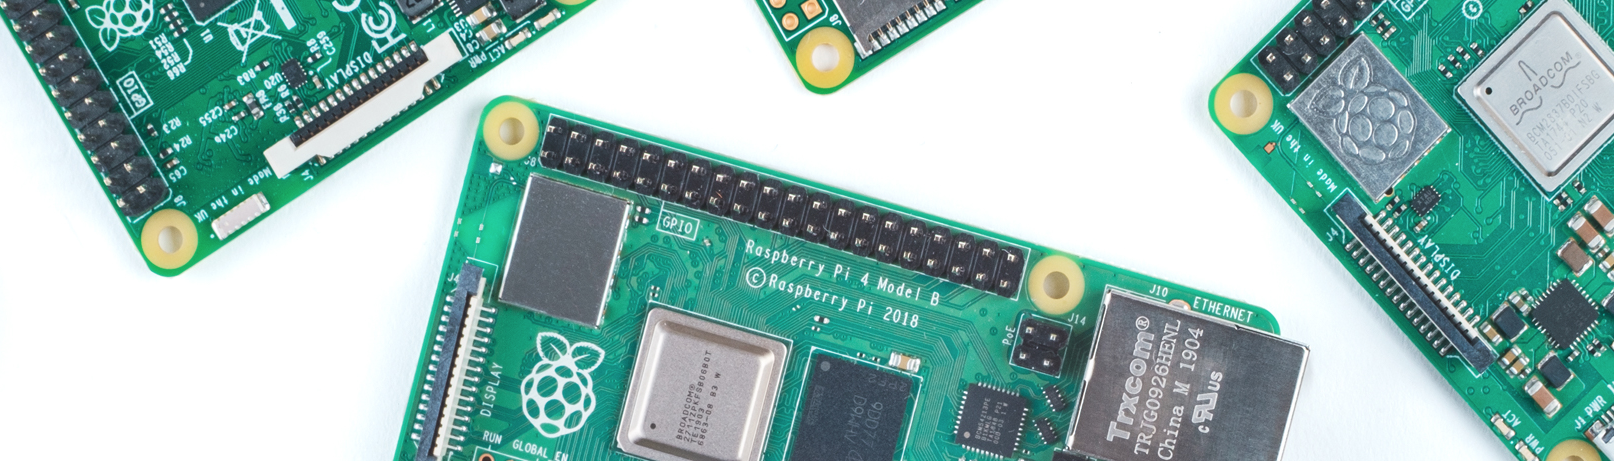
\includegraphics[width=1\linewidth]{images/raspberrypi} 

}

\caption{An abundance of free software and relatively cheap new hardware like the \href{https://www.raspberrypi.org}{Raspberry Pi} \citep{raspberrypi}, \href{https://microbit.org}{Microbit}, \citep{Sentance2017} \href{https://makeymakey.com}{Makey Makey} {[}\citet{nevertooold}; \citet{makeymakey};{]} \href{https://redfernelectronics.co.uk/crumble/}{Crumble Controller} and \href{https://www.arduino.cc}{Arduino} \citep{arduino} has opened up lots of new possibilities for teaching Computer Science. Picture via Alex Bate. \citep{SnazzyRPi})}\label{fig:unnamed-chunk-7}
\end{figure}

Our aim is to support the teaching and learning of Computer Science in your school and to help engage schoolchildren in the subject. This page describes what we can provide you with and what we expect to get in return.

\hypertarget{what-the-university-is-offering-your-school}{%
\subsection{What the University is offering your school}\label{what-the-university-is-offering-your-school}}

The University of Manchester will provide your school or college with at least one student ambassador with some relevant training who has completed two years of study in Computer Science and has:

\begin{itemize}
\tightlist
\item
  A good knowledge of, and enthusiasm for Computer Science
\item
  Completed \href{https://www.gov.uk/government/organisations/disclosure-and-barring-service}{Disclosure and Barring Service} (DBS) clearance
\item
  An interest in teaching and working with young people
\item
  Achieved a minimum of a 2:1 or 1st class degree in their second year
\end{itemize}

\hypertarget{what-the-university-expects-from-your-school}{%
\subsection{What the University expects from your school}\label{what-the-university-expects-from-your-school}}

In return, we expect that the school provides the undergraduate student with:

\begin{itemize}
\tightlist
\item
  Opportunities to engage with a classroom or after school club of children as a Teaching Assistant (TA). This is typically for around one or two hours during term time. Initially, this could be through classroom observation and teacher assistance, culminating in the student delivering at least one lesson (and potentially a series of lessons) with your support and guidance
\item
  Advice, suggestions, feedback, assessment and encouragement from you to suggest the kinds of resources that would be useful, appropriate or engaging for the Computer Science curriculum you are teaching
\item
  Classroom and behaviour management: the students are not trained teachers and will be relying on your expertise in classroom and behaviour management.
\end{itemize}

\hypertarget{resources-developed-by-students}{%
\subsection{Resources developed by students}\label{resources-developed-by-students}}

Undergraduates typically develop a range of resources. The project will involve development of a computer-based system together with supporting activities, lessons and resources. The resource could be a variety of things including, a game, robotics, animations, hardware (Raspberry Pi, Arduino etc) or software, intended to enthuse school students at one of the Key stages 3 or 4 about fundamental concepts in computing preferably linked to one of the new Computer Science curricula.

\hypertarget{project-timing}{%
\subsection{Project timing}\label{project-timing}}

The projects run for 6 months from September to March, divided into three phases.

\begin{enumerate}
\def\labelenumi{\arabic{enumi}.}
\tightlist
\item
  \textbf{September to October} Observation in the classroom teaching by the student around once per week. Development of ideas for an educational tool that the student will make, with the advice of the classroom teacher
\item
  \textbf{November to January} From November to January, our students develop and tests prototype tool (or tools) with the supporting material, this can happen sooner for students who make a quick start to the project.
\item
  \textbf{February to April} From February to April, our students are expected to liaise closely with teachers to develop an educational tool that will be of use in the classroom using teachers' suggestions as to what is appropriate to build. Students will spend some time in a classroom working closely with teachers and students developing and delivering a new resource for teaching. More details on final year projects can be found in COMP300, the undergraduates already know what is required from their project
\end{enumerate}

\hypertarget{assessment-and-monitoring}{%
\subsection{Assessment and monitoring}\label{assessment-and-monitoring}}

Formal supervision and mentoring is undertaken by the university (Duncan and David), but we will ask you to fill in a one page form on your assessment of their progress during their time at your school, we very much value your input and hope that these projects can beneficial for both your school and the University. We don't want to burden you with unnecessary bureaucracy that all teachers battle with!

\hypertarget{guidance-for-students}{%
\section{Guidance for students}\label{guidance-for-students}}

\begin{figure}

{\centering 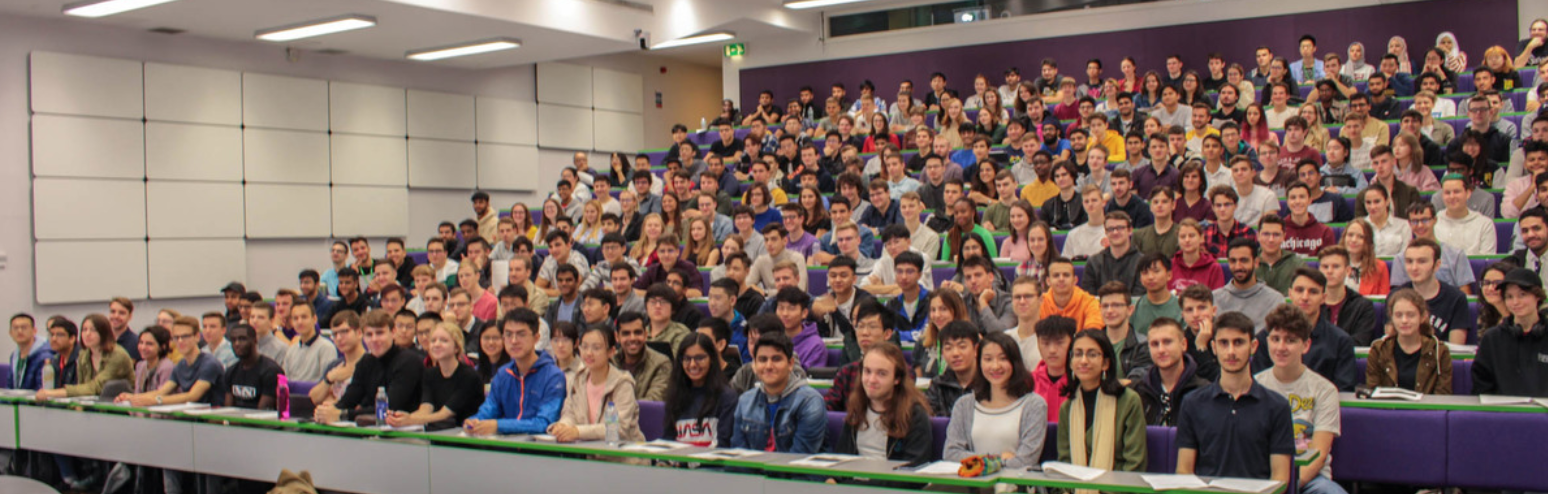
\includegraphics[width=1\linewidth]{images/studentspanorama} 

}

\caption{Lecture theatre 1.1 (LT 1.1) in Kilburn full of first year students}\label{fig:unnamed-chunk-8}
\end{figure}

So why would you, an undergraduate student, want to work on an education project in secondary school? The UK government would like Computer Science should be taught in all secondary schools in the UK. \citep{afterthereboot} However, in many UK schools there is a shortage of teachers who are trained in Computer Science, consequently, many teachers find themselves being asked to teach a subject they may know little about. \citep{shutdownrestart}

Undergraduate students can make a significant difference here, by supporting teachers in the classroom to create and deliver new classroom resources in Computer Science. \citep{computinged} In addition, undergraduate students will have the chance to:

\begin{itemize}
\tightlist
\item
  develop leadership skills in the classroom
\item
  gain valuable experience of working on ``real world'' problems in a stimulating environment
\item
  improve your communication skills, especially spoken communication
  work as part of a team (in the school) and join a small group of like-minded undergraduate students (in the University) working on related projects
\item
  test your knowledge \& technical ability in a challenging and dynamic environment working with young people
\item
  last, but not least, there is a good chance you will have lots of fun and have a rewarding experience of teaching
  make yourself more employable by doing all of the above
\end{itemize}

\hypertarget{who-is-involved}{%
\subsection{Who is involved?}\label{who-is-involved}}

Initially, the number of undergraduate students involved in these projects will be less than ten. We also require that you will have a minimum of a 2:1 or 1st in your second year exams. Projects are co-supervised by Duncan with additional supervision from an experienced member of teaching staff at a participating school.

We have carefully selected schools in Manchester that are relatively easy for you to get to, are already teaching Computer Science and have supportive staff and teachers in place to help you. You will be expected to work directly with school children with the support of the teaching staff in your school. Schools we have worked with are all the Manchester area.

\hypertarget{what-will-the-educational-projects-be-expected-to-deliver}{%
\subsection{What will the educational projects be expected to deliver?}\label{what-will-the-educational-projects-be-expected-to-deliver}}

You will be expected to work closely with the teacher to develop resources that

\begin{itemize}
\tightlist
\item
  engage students with one or more aspects of the new Computer Science curriculum at an appropriate key stage. This is usually \href{https://en.wikipedia.org/wiki/Key_Stage_3}{key stage 3}, \href{https://en.wikipedia.org/wiki/Key_Stage_4}{key stage 4} or \href{https://en.wikipedia.org/wiki/Key_Stage_5}{key stage 5} ages 11-18.
\item
  complement \textbf{and extend} the schools current provision for computer science in the school
\end{itemize}

During the project you will be spending a significant amount of time in the classroom, visiting your school every week during school term time throughout the duration of your project to develop resources. These must include a computer-based teaching tool which may use, for example, Raspberry Pi's, visual aids, demonstrations, videos, online questionnaires, formative feedback, games, drones, robotics, music, \citep{Aaron2016} algorithms \citep{Kubica2012} or even just the command line \citep{conquerthecommandline} etc.\footnote{Conquer the command line is part of the The MagPi essentials series, there are lots of others like it you may find useful on using the camera module, gaming in python, simple electronics and more at \url{https://store.rpipress.cc}} In addition, guidance on classroom use, such as a lesson or series of lessons to support the tool. Remember that you don't actually need a computer, see \href{https://csunplugged.org}{Computer Science Unplugged}: Computer Science without a Computer. \citep{Bell2018}

All deliverables for standard final year projects will be expected of these projects including:

\begin{itemize}
\tightlist
\item
  first semester presentation
\item
  demonstration of the resource being used in the classroom
\item
  final written report
\end{itemize}

Assessments for these projects will be as for standard projects, \citep{COMP30030, COMP30040} but part of the evaluation of the project will be a classroom demonstration, a description and evaluation of which should be included in your final report.

\hypertarget{getting-a-head-start}{%
\subsection{Getting a head start}\label{getting-a-head-start}}

There are plenty of online courses you can do to improve you effectiveness in the classroom.

\begin{itemize}
\tightlist
\item
  Impact of Technology: How To Lead Classroom Discussions. Learn how to keep 14-16 year-old students engaged in discussions while teaching computer science. Supported by Google \href{https://www.futurelearn.com/courses/impact-of-technology}{futurelearn.com/courses/impact-of-technology}
\item
  Teaching Physical Computing with Raspberry Pi and Python \href{https://www.futurelearn.com/courses/physical-computing-raspberry-pi-python}{futurelearn.com/courses/physical-computing-raspberry-pi-python}
\item
  Since some of your teaching is likely to be asynchronous, you would also benefit from having a look at \href{https://www.open.edu/openlearn/education-development/education/take-your-teaching-online/content-section-overview}{taking your teaching online} from OpenLearn
\item
  Many more Teaching Computing Courses at \href{https://www.futurelearn.com/subjects/teaching-courses/teaching-computing}{futurelearn.com/subjects/teaching-courses/teaching-computing}
\end{itemize}

\hypertarget{blended}{%
\subsection{Blended learning}\label{blended}}

COVID 19 is revolutionising teaching, from primary and secondary school right through to higher education. You need to get clued up on \href{https://en.wikipedia.org/wiki/Blended_learning}{blended learning}. Start with \href{http://www.elearning.fse.manchester.ac.uk/fseta/moving-to-blended-learning-part-1-terminology-and-concepts/}{Moving to Blended Learning, Part 1: Terminology and Concepts}, then take a look the video below with Steve Pettifer explaining techniques for slides that work for blended learning videos:

When you teach, think about how you can support students before and after your time in the classroom.

\hypertarget{finishing}{%
\subsection{When do the projects start and finish?}\label{finishing}}

Projects start annually in September and are handed at Easter time, see final year project guidelines. For more information contact \protect\hyperlink{Contact}{Duncan Hull}.

\hypertarget{contact}{%
\chapter{Contact}\label{contact}}

You can get in touch using the details below, which include directions and parking information.



\begin{figure}

{\centering 
\includegraphics[width=1\linewidth]{images/turingicon} 

}

\caption{Paying homage to \href{https://en.wikipedia.org/wiki/Alan_Turing}{Alan Turing} at a mural on the \href{https://en.wikipedia.org/wiki/A5103_road}{Princess Parkway} by \href{http://tankpetrol.com/}{tankpetrol.com}. Turing is, as \href{https://www.manturing.net/jonathan}{Jonathan Swinton} puts it, the ``patron saint of Manchester'' \citep{manturing}. As a \href{https://en.wikipedia.org/wiki/Symbols_of_Manchester}{Manchester icon}, he is commemorated locally by the \href{https://en.wikipedia.org/wiki/Alan_Turing_Building}{Alan Turing building}, the \href{https://en.wikipedia.org/wiki/Alan_Turing_Memorial}{Alan Turing Memorial} and Alan Turing Way \citep{turingway}}\label{fig:unnamed-chunk-9}
\end{figure}

\hypertarget{office}{%
\section{Office}\label{office}}

Our offices are in the Kilburn building, close to the Byte cafe, past the \href{https://studentnet.cs.manchester.ac.uk/student-services/}{Student Support Office} (SSO), through the double doors, down the ramp.

\textbf{Dr.~Duncan Hull, Lecturer} 👨‍💻

\begin{itemize}
\tightlist
\item
  🏢 Room LF25, Kilburn Building
\item
  📥 email: duncan.hull ATE manchester.ac.uk
\item
  ☎️ telephone: +44 161 275 6186
\item
  🌐 \href{https://uk.linkedin.com/in/duncanhull}{linkedin.com/in/duncanhull}
\end{itemize}

\textbf{Mabel Yau, Careers and placements officer} 👩‍💻

\begin{itemize}
\tightlist
\item
  🏢 Room LF26, Kilburn Building
\item
  📥 email: mabel.yau ATE manchester.ac.uk
\item
  ☎️ telephone: +44 161 275 6140
\item
  🌐 \href{https://uk.linkedin.com/in/mabel-yau}{linkedin.com/in/mabel-yau}
\end{itemize}

\textbf{Student Support Office } 👨‍👩‍👧‍👧

\begin{itemize}
\tightlist
\item
  🏢 Room LF21, Kilburn Building
\item
  📥 email \href{mailto:compsci-sso@manchester.ac.uk}{\nolinkurl{compsci-sso@manchester.ac.uk}}
\item
  ☎️ telephone: +44 161 306 8155
\end{itemize}

\hypertarget{video-conferencing}{%
\section{Video conferencing}\label{video-conferencing}}

The University of Manchester has an enterprise subscription for Zoom and Microsoft Teams. For the latter, you can contact me using \href{https://zoom.us/my/duncanhull}{zoom.us/my/duncanhull}. For most other enterprise video conferencing software, your employer will need to host the meeting and send me an invitation link. Please provide any log in, dial in, invitation links or meeting IDs for:

\begin{itemize}
\tightlist
\item
  \href{https://en.wikipedia.org/wiki/Skype_for_Business}{Skype for business}
\item
  \href{https://en.wikipedia.org/wiki/BlueJeans}{Bluejeans}
\item
  \href{https://en.wikipedia.org/wiki/Microsoft_Teams}{Microsoft Teams}
\item
  \href{https://en.wikipedia.org/wiki/Cisco_Webex}{Cisco Webex}
\end{itemize}

You can also contact me using free versions of:

\begin{itemize}
\tightlist
\item
  \href{https://aws.amazon.com/chime/}{Amazon Chime}
\item
  \href{https://en.wikipedia.org/wiki/Discord_(software)}{Discord}
\item
  \href{https://en.wikipedia.org/wiki/Slack_(software)}{Slack}
\item
  \href{https://en.wikipedia.org/wiki/Skype}{Skype} (the non-business version where my username is ``duncanhull'')
\item
  \href{https://en.wikipedia.org/wiki/Jitsi}{Jitsi}
\item
  \href{https://en.wikipedia.org/wiki/Google_Hangouts}{Google Hangouts} Google id is my University email address
\end{itemize}

\hypertarget{online-and-social-media}{%
\section{Online and social media}\label{online-and-social-media}}

You can get in touch via t'internet at:

\begin{itemize}
\tightlist
\item
  Blog: \href{https://duncan.hull.name}{duncan.hull.name}
\item
  Github: \href{https://github.com/dullhunk}{github.com/dullhunk}
\item
  Twitter: \href{https://twitter.com/dullhunk}{twitter.com/dullhunk}
\end{itemize}

\hypertarget{postal-address}{%
\section{Postal address}\label{postal-address}}

Send post by snail mail 🐌 to :

Dr.~Duncan Hull\\
Lecturer\\
Department of Computer Science\\
Kilburn Building\\
The University of Manchester\\
Oxford Road\\
Manchester\\
M13 9PL\\
\href{https://duncan.hull.name/2019/07/05/mancashire/}{Lancashire} 🌹

\hypertarget{kilburn-building-directions}{%
\section{Kilburn building directions}\label{kilburn-building-directions}}

From the train stations, it takes about 20 minutes to walk from \href{https://www.nationalrail.co.uk/stations_destinations/man.aspx}{Manchester Piccadilly} (MAN) and ten minutes from \href{https://www.nationalrail.co.uk/stations/mco/details.aspx}{Manchester Oxford Road} (MCO). Our official postcode (M13 9PL) takes you to \href{http://www.conference.manchester.ac.uk/venues/search/details/?property=10}{University Place} next door, so you're better of using the \href{https://www.bbc.co.uk/news/uk-england-49319760}{what3words locations} \citep{what3words} below which are more accurate:

\begin{itemize}
\tightlist
\item
  Google map of the Kilburn building \href{http://bit.ly/directions-to-kilburn-building}{bit.ly/directions-to-kilburn-building}
\item
  There are two ground floor entrances to the Kilburn building, North and South

  \begin{itemize}
  \tightlist
  \item
    North entrance: \href{https://what3words.com/port.museum.rips}{what3words.com/port.museum.rips}
  \item
    South entrance: \href{https://what3words.com/common.wiping.email}{what3words.com/common.wiping.email}
  \end{itemize}
\item
  There is no formal reception so the best place to meet is \href{http://bit.ly/ByteCafe}{bit.ly/ByteCafe} on the first floor
\item
  See also \href{https://www.cs.manchester.ac.uk/about/maps-and-travel/}{cs.manchester.ac.uk/about/maps-and-travel/}
\end{itemize}

\hypertarget{parking}{%
\section{Parking}\label{parking}}

If you are driving, the nearest car parks are:

\begin{itemize}
\tightlist
\item
  \textbf{University Car Park B} \href{https://www.ncp.co.uk/find-a-car-park/car-parks/manchester-aquatic-centre-jv/}{Manchester Aquatics Centre Car Park}, NCP \href{http://maps.google.co.uk/maps?q=M13+9SS}{M13 9SS}
\item
  \textbf{University Car Park D} Booth Street West Car Park, \href{http://maps.google.co.uk/maps?q=M15+6AR}{M15 6AR}, access via Higher Cambridge Street
\item
  See \href{https://www.estates.manchester.ac.uk/services/operationalservices/carparking/}{estates.manchester.ac.uk/services/operationalservices/carparking}
\end{itemize}

\hypertarget{appendix-appendix}{%
\appendix}


\hypertarget{referee}{%
\chapter{Will you write a reference for me?}\label{referee}}

As employability tutor, I get asked to write \emph{lots} references for students applying for jobs and further study. I'm happy to do this if you've been personal tutee or I've worked with you outside of ordinary teaching. However, it's impossible to for me to say YES to every request for a reference. For students I haven't worked with, it is difficult to do, because all I can confirm is facts (attendance, academic marks, degree program) without opinions which doesn't make for a very compelling reference.

Whoever agrees to be your referee, make sure you read and understand the following:

\hypertarget{who-can-provide-a-reference-for-me}{%
\section{Who can provide a reference for me?}\label{who-can-provide-a-reference-for-me}}

The best person to provide a reference for you is somebody who knows you, such as your personal tutor. See the careers service guide \href{http://www.careers.manchester.ac.uk/applicationsinterviews/faqs/references}{what are references and how should I choose a referee?} and \href{http://documents.manchester.ac.uk/display.aspx?DocID=1921}{guidance to staff providing references for students} from the University of Manchester, which gives extra context.

It is good to have references from different sources, so if you are providing several referees try to pick people from inside and outside the University. Within the University, this is most likely to be your tutor:

\begin{itemize}
\tightlist
\item
  Your personal tutor from year one
\item
  Your personal tutor from year two (if different to first year)
\item
  Your IE tutor (mostly likely me)
\item
  Your third year project supervisor
\item
  Anyone else who knows you personally
\end{itemize}

If you ask somebody who does not know you very well to write a reference for you, all that they are able to do in a reference is confirm rather dull facts such as your grades, your attendance, start date and graduation date. As I've already said, this does not make for a very useful reference.

\hypertarget{should-i-ask-permission-from-my-referee}{%
\section{Should I ask permission from my referee?}\label{should-i-ask-permission-from-my-referee}}

You should always ask the person providing your reference.

\hypertarget{what-is-a-reference-for}{%
\section{What is a reference for?}\label{what-is-a-reference-for}}

References have two main purposes:

\begin{enumerate}
\def\labelenumi{\arabic{enumi}.}
\tightlist
\item
  Providing and confirming \emph{facts}

  \begin{enumerate}
  \def\labelenumii{\roman{enumii}.}
  \tightlist
  \item
    to give a factual account, e.g.~of academic record, attendance, etc
  \item
    to confirm the accuracy of statements made in an application
  \end{enumerate}
\item
  Providing \emph{opinions}

  \begin{enumerate}
  \def\labelenumii{\roman{enumii}.}
  \tightlist
  \item
    to give the referee's opinion as to the candidate's suitability for the post/course in
    question, and his/her potential for the future
  \end{enumerate}
\end{enumerate}

\hypertarget{how-can-i-help-my-referee}{%
\section{How can I help my referee?}\label{how-can-i-help-my-referee}}

It can make it much easier for your referee if you provide them with information you would like them to mention in your reference. This might include information about your character, projects you have completed or specific aspects of your academic performance. Providing an up to date CV also helps your referee.

\hypertarget{can-i-have-a-copy-of-my-reference}{%
\section{Can I have a copy of my reference?}\label{can-i-have-a-copy-of-my-reference}}

It is unusual for a referee to provide a reference directly to its subject (that's you).

Typically, a referee is asked to provide a reference for a student (or former student) directly by the organisation concerned. For example, if you're applying for postgraduate study, the reference request will be sent by the University directly to your referees email address, who will usually respond by clicking on a link to upload the reference document.

You can make a request to see your reference under data protection law.

  \bibliography{hulld.bib}

\end{document}
